\chapter{Chapter 1}
\minitoc
\label{chap:1st}
\section*{Introduction}
    This chapter delves into ....

\section{Template}
    \subsection{References}
        This is how you reference the webography \cite{web:melek} and bibliography \cite{ref:example}.
        
    \subsection{Equations}
        This is an example equation: \ref{equ:example}.

       \begin{equation}
            \text{Accuracy} = \frac{\text{TP} + \text{TN}}{\text{TP} + \text{TN} + \text{FP} + \text{FN}}
            \label{equ:example}
        \end{equation}


        

        
    \subsection{Figures}
        This is an example of a single image figure \ref{img:single}.

        \begin{figure}[htbp]
        \centerline{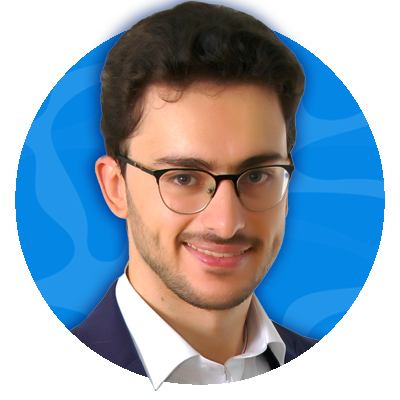
\includegraphics[width=0.9\textwidth]{images/example.png}}
        \caption{Single image}
        \label{img:single}   
        \end{figure}

        This is an example of a multiple image figure \ref{img:multiple}
        
        \begin{figure}[htbp]
        \begin{subfigure}[t]{0.5\linewidth}
        \centering
        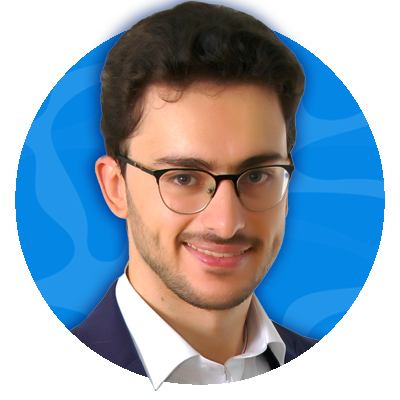
\includegraphics[width=0.7\textwidth]{images/example.png}
        \caption{Image 1}
        \label{subfig:img1}
        \end{subfigure}%
        \begin{subfigure}[t]{0.5\linewidth}
        \centering
        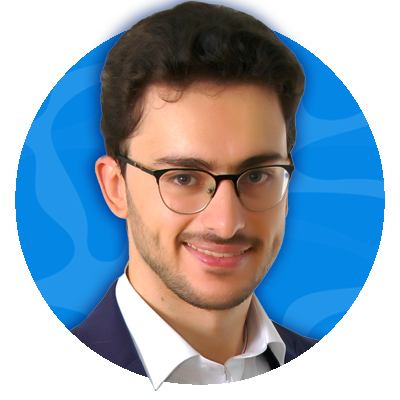
\includegraphics[width=0.7\textwidth]{images/example.png}
        \caption{Image 2}
        \label{subfig:img2}
        \end{subfigure}
        \caption{Multiple images}
        \label{img:multiple}
        \end{figure}
        
        
    \subsection{Tables}
        This is an example of a simple table \ref{tab:simple}

        \begin{table}[H]
        \centering
        \scalebox{1}{
        \begin{tabular}{|l|c|c|}
        \hline
        \textbf{x} & \textbf{y} & \textbf{z} \\
        \hline
        \textbf{a} & 5 & \cellcolor{green!10}7  \\
        \hline
        \textbf{b} & 63 & \cellcolor{green!10}8  \\
        \hline
        \end{tabular}
        }
        \caption{Simple table}
        \label{tab:simple}
        \end{table}

        This is an example of a complex table \ref{tab:complex}
        
        \begin{table}[htbp]
        \begin{center}
        
        \begin{tabular}{|c|l|c|c|c|}
        \cline{3-5}
        \multicolumn{2}{c|}{}&\multicolumn{3}{|c|}{\textbf{metric(\%)$\uparrow$}}\\
        \cline{2-5}
        \multicolumn{1}{c|}{}&\textbf{a} & train & valid & test  \\
        \hline
        
        \parbox[t]{2mm}{\multirow{2}{*}{\rotatebox[origin=c]{90}{\textbf{bc}}}}
        & b      &   5   &   5  &   5  \\
        & c      &   5   &   5  &   5  \\
        \hline
        \hline
        
        \parbox[t]{2mm}{\multirow{2}{*}{\rotatebox[origin=c]{90}{\textbf{de}}}} 
        & d      &   5  &   5   &   5  \\
        & e            &   5   &   5   &   5  \\
        \hline
        \hline   

        \rowcolor{gray!10}&\textbf{f} &   \textbf{10}   &   \textbf{10}   &   \textbf{10} \\
        \hline
        
        \end{tabular}
        \caption{Complex table}
        \label{tab:complex}
        \end{center}
        \end{table}


        
\section*{Conclusion}
    We presented ....